\documentclass[12pt,letterpaper]{article}
%\documentstyle[11pt]{article}
\usepackage[utf8]{inputenc}
\usepackage{amsmath}
\usepackage{xfrac}
\usepackage{amsfonts}
\usepackage{amssymb}
\usepackage[version = 3]{mhchem}
\usepackage{chemstyle}
%%For Table perhaps%%
%\usepackage{graphics}
\usepackage{graphicx}
\usepackage{epstopdf}
\usepackage{tabularx,ragged2e,booktabs,caption}
%\newcolumntype{C}[1]{>{\Centering}m{#1}}
%\renewcommand\tabularxcolumn[1]{C{#1}}
\usepackage[left=1.5cm,right=1.5cm,top=0.5cm,bottom=2cm]{geometry}
\usepackage{subcaption} 
\usepackage{caption}
\usepackage[colorlinks]{hyperref}
\usepackage[svgnames]{xcolor}
\hypersetup{citecolor=DeepPink4}
\hypersetup{linkcolor=DarkRed}
\hypersetup{urlcolor=DarkBlue}
\usepackage{cleveref}

\begin{document}
\setlength{\parindent}{0cm} 


\frenchspacing


\title {\large{\textbf{Quiz 6---Microbial Growth}}\\ \large{CENG 340--Introduction to Environmental Engineering\\
Instructor: Deborah Sills, \textbf{15 November, 2013}}}
\author {}
\date {}
\maketitle

\vspace{-0.5 in}
\textbf{\large{Name:}}\\


Environmental engineers use a mixed-order kinetic model (the Monod model), described by Eq.1 and presented in Fig. 1, to estimate the net growth rate of bacteria in biological treatment reactors.  

\begin{align}
\mathrm{\frac{dX}{dt} = \frac{\mu_{max}XS}{K_s + S}}
\end{align}

\begin{figure}
\centering
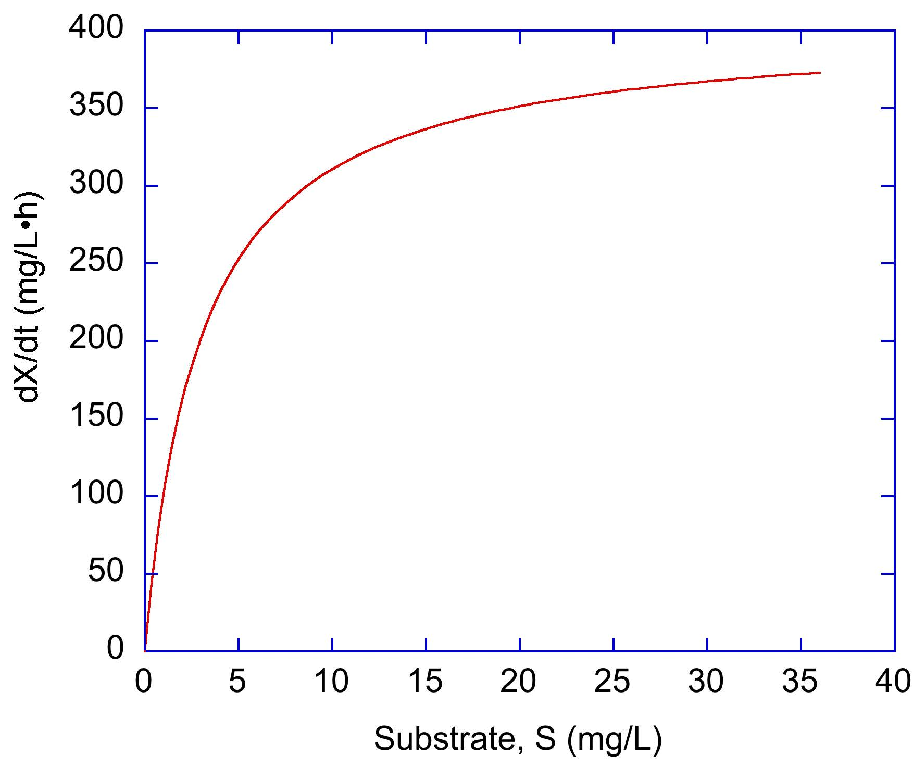
\includegraphics[width=0.4\textwidth]{monod}
\caption{Net growth rate of microroganisms as a function of substrate concentration.}
\end{figure}

\begin{enumerate}
\item \emph{(5 pts)} Describe very briefly under what conditions the growth rate ($\mathrm{\frac{dX}{dt}}$) is zero order with respect to S, and write the resulting zero-order rate equation.

\vspace{1.3in}

\item \emph{(5 pts)} Describe very briefly under what conditions the growth rate ($\mathrm{\frac{dX}{dt}}$) is first order with respect to S, and write the resulting first-order rate equation.



%\item The substrate utilization kinetics of a bacterium has been characterized and obey the following mixed-order relationship.
%
%\begin{align*}
%\mathrm{\frac{\frac{dS}{dt}}{X} = - \frac{24S}{6 + S}}
%\end{align*}
%
%At what substrate concentration, S, will the specific utilization rate $\mathrm{\frac{\frac{dS}{dt}}{X}}$ be one-half of its maximum value.
%\end{enumerate}
\end{enumerate}


\vspace{-0.1in}







\end{document}